\documentclass[letterpaper]{article}
%\documentclass[a5paper]{article}

%% Language and font encodings
\usepackage[english]{babel}
\usepackage[utf8x]{inputenc}
\usepackage[T1]{fontenc}

%% Sets page size and margins
\usepackage[letterpaper,top=1in,bottom=1in,left=1in,right=1in,marginparwidth=1.75cm]{geometry}
%\usepackage[a5paper,top=1cm,bottom=1cm,left=1cm,right=1.5cm,marginparwidth=1.75cm]{geometry}

\usepackage{graphicx}
%\graphicspath{../images}	  %%where to look for images

%% Useful packages
\usepackage{amssymb, amsmath, amsthm} 
%\usepackage{graphicx}  %%this is currently enabled in the default document, so it is commented out here. 
\usepackage{calrsfs}
\usepackage{braket}
\usepackage{mathtools}
\usepackage{lipsum}
\usepackage{tikz}
\usetikzlibrary{cd}
\usepackage{verbatim}
%\usepackage{ntheorem}% for theorem-like environments
\usepackage{mdframed}%can make highlighted boxes of text
%Use case: https://tex.stackexchange.com/questions/46828/how-to-highlight-important-parts-with-a-gray-background
\usepackage{wrapfig}
\usepackage{centernot}
\usepackage{subcaption}%\begin{subfigure}{0.5\textwidth}
\usepackage{pgfplots}
\pgfplotsset{compat=1.13}
\usepackage[colorinlistoftodos]{todonotes}
\usepackage[colorlinks=true, allcolors=blue]{hyperref}
\usepackage{xfrac}					%to make slanted fractions \sfrac{numerator}{denominator}
\usepackage{enumitem}            
    %syntax: \begin{enumerate}[label=(\alph*)]
    %possible arguments: f \alph*, \Alph*, \arabic*, \roman* and \Roman*
\usetikzlibrary{arrows,shapes.geometric,fit}

\DeclareMathAlphabet{\pazocal}{OMS}{zplm}{m}{n}
%% Use \pazocal{letter} to typeset a letter in the other kind 
%%  of math calligraphic font. 

%% This puts the QED block at the end of each proof, the way I like it. 
\renewenvironment{proof}{{\bfseries Proof}}{\qed}
\makeatletter
\renewenvironment{proof}[1][\bfseries \proofname]{\par
  \pushQED{\qed}%
  \normalfont \topsep6\p@\@plus6\p@\relax
  \trivlist
  %\itemindent\normalparindent
  \item[\hskip\labelsep
        \scshape
    #1\@addpunct{}]\ignorespaces
}{%
  \popQED\endtrivlist\@endpefalse
}
\makeatother

%% This adds a \rewnewtheorem command, which enables me to override the settings for theorems contained in this document.
\makeatletter
\def\renewtheorem#1{%
  \expandafter\let\csname#1\endcsname\relax
  \expandafter\let\csname c@#1\endcsname\relax
  \gdef\renewtheorem@envname{#1}
  \renewtheorem@secpar
}
\def\renewtheorem@secpar{\@ifnextchar[{\renewtheorem@numberedlike}{\renewtheorem@nonumberedlike}}
\def\renewtheorem@numberedlike[#1]#2{\newtheorem{\renewtheorem@envname}[#1]{#2}}
\def\renewtheorem@nonumberedlike#1{  
\def\renewtheorem@caption{#1}
\edef\renewtheorem@nowithin{\noexpand\newtheorem{\renewtheorem@envname}{\renewtheorem@caption}}
\renewtheorem@thirdpar
}
\def\renewtheorem@thirdpar{\@ifnextchar[{\renewtheorem@within}{\renewtheorem@nowithin}}
\def\renewtheorem@within[#1]{\renewtheorem@nowithin[#1]}
\makeatother

%% This makes theorems and definitions with names show up in bold, the way I like it. 
\makeatletter
\def\th@plain{%
  \thm@notefont{}% same as heading font
  \itshape % body font
}
\def\th@definition{%
  \thm@notefont{}% same as heading font
  \normalfont % body font
}
\makeatother

%===============================================
%==============Shortcut Commands================
%===============================================
\newcommand{\ds}{\displaystyle}
\newcommand{\B}{\mathcal{B}}
\newcommand{\C}{\mathbb{C}}
\newcommand{\F}{\mathbb{F}}
\newcommand{\N}{\mathbb{N}}
\newcommand{\R}{\mathbb{R}}
\newcommand{\Q}{\mathbb{Q}}
\newcommand{\T}{\mathcal{T}}
\newcommand{\Z}{\mathbb{Z}}
\renewcommand\qedsymbol{$\blacksquare$}
\newcommand{\qedwhite}{\hfill\ensuremath{\square}}
\newcommand*\conj[1]{\overline{#1}}
\newcommand*\closure[1]{\overline{#1}}
\newcommand*\mean[1]{\overline{#1}}
%\newcommand{\inner}[1]{\left< #1 \right>}
\newcommand{\inner}[2]{\left< #1, #2 \right>}
\newcommand{\powerset}[1]{\pazocal{P}(#1)}
%% Use \pazocal{letter} to typeset a letter in the other kind 
%%  of math calligraphic font. 
\newcommand{\cardinality}[1]{\left| #1 \right|}
\newcommand{\domain}[1]{\mathcal{D}(#1)}
\newcommand{\image}{\text{Im}}
\newcommand{\inv}[1]{#1^{-1}}
\newcommand{\preimage}[2]{#1^{-1}\left(#2\right)}
\newcommand{\script}[1]{\mathcal{#1}}


\newenvironment{highlight}{\begin{mdframed}[backgroundcolor=gray!20]}{\end{mdframed}}

\DeclarePairedDelimiter\ceil{\lceil}{\rceil}
\DeclarePairedDelimiter\floor{\lfloor}{\rfloor}

%===============================================
%===============My Tikz Commands================
%===============================================
\newcommand{\drawsquiggle}[1]{\draw[shift={(#1,0)}] (.005,.05) -- (-.005,.02) -- (.005,-.02) -- (-.005,-.05);}
\newcommand{\drawpoint}[2]{\draw[*-*] (#1,0.01) node[below, shift={(0,-.2)}] {#2};}
\newcommand{\drawopoint}[2]{\draw[o-o] (#1,0.01) node[below, shift={(0,-.2)}] {#2};}
\newcommand{\drawlpoint}[2]{\draw (#1,0.02) -- (#1,-0.02) node[below] {#2};}
\newcommand{\drawlbrack}[2]{\draw (#1+.01,0.02) --(#1,0.02) -- (#1,-0.02) -- (#1+.01,-0.02) node[below, shift={(-.01,0)}] {#2};}
\newcommand{\drawrbrack}[2]{\draw (#1-.01,0.02) --(#1,0.02) -- (#1,-0.02) -- (#1-.01,-0.02) node[below, shift={(+.01,0)}] {#2};}

%***********************************************
%**************Start of Document****************
%***********************************************

%===============================================
%===============Theorem Styles==================
%===============================================

%================Default Style==================
\theoremstyle{plain}% is the default. it sets the text in italic and adds extra space above and below the \newtheorems listed below it in the input. it is recommended for theorems, corollaries, lemmas, propositions, conjectures, criteria, and (possibly; depends on the subject area) algorithms.
\newtheorem{theorem}{Theorem}
\numberwithin{theorem}{section} %This sets the numbering system for theorems to number them down to the {argument} level. I have it set to number down to the {section} level right now.
\newtheorem*{theorem*}{Theorem} %Theorem with no numbering
\newtheorem{corollary}[theorem]{Corollary}
\newtheorem*{corollary*}{Corollary}
\newtheorem{conjecture}[theorem]{Conjecture}
\newtheorem{lemma}[theorem]{Lemma}
\newtheorem*{lemma*}{Lemma}
\newtheorem{proposition}[theorem]{Proposition}
\newtheorem*{proposition*}{Proposition}
\newtheorem{problemstatement}[theorem]{Problem Statement}


%==============Definition Style=================
\theoremstyle{definition}% adds extra space above and below, but sets the text in roman. it is recommended for definitions, conditions, problems, and examples; i've alse seen it used for exercises.
\newtheorem{definition}[theorem]{Definition}
\newtheorem*{definition*}{Definition}
\newtheorem{condition}[theorem]{Condition}
\newtheorem{problem}[theorem]{Problem}
\newtheorem{example}[theorem]{Example}
\newtheorem*{example*}{Example}
\newtheorem*{counterexample*}{Counterexample}
\newtheorem*{romantheorem*}{Theorem} %Theorem with no numbering
\newtheorem{exercise}{Exercise}
\numberwithin{exercise}{section}
\newtheorem{algorithm}[theorem]{Algorithm}

%================Remark Style===================
\theoremstyle{remark}% is set in roman, with no additional space above or below. it is recommended for remarks, notes, notation, claims, summaries, acknowledgments, cases, and conclusions.
\newtheorem{remark}[theorem]{Remark}
\newtheorem*{remark*}{Remark}
\newtheorem{notation}[theorem]{Notation}
\newtheorem*{notation*}{Notation}
%\newtheorem{claim}[theorem]{Claim}  %%use this if you ever want claims to be numbered
\newtheorem*{claim}{Claim}



\pgfplotsset{compat=1.13}

\newcommand{\T}{\mathcal{T}}
\newcommand{\B}{\mathcal{B}}
\newcommand{\arbcup}[1]{\bigcup\limits_{\alpha\in\Gamma}#1_\alpha}
\newcommand{\arbcap}[1]{\bigcap\limits_{\alpha\in\Gamma}#1_\alpha}
\newcommand{\Rbad}{\R_\text{bad}}

\title{Math 501 \linebreak
Homework 5}
\author{Trevor Klar}

\begin{document}

\maketitle


\begin{enumerate}
\item Let $S^1=\{(x,y):x^2+y^2=1\}$ denote the unit circle in $\R^2$. Let $f:[0,1)\to S^1$ be $f(t) = (\cos{2\pi t}, \sin{2\pi t})$. Show that $f$ is not a homeomorphism. 
\begin{proof}
Let $U=B((1,0),1)\cap S^1$. 

\begin{figure}[h]
  \begin{center}
    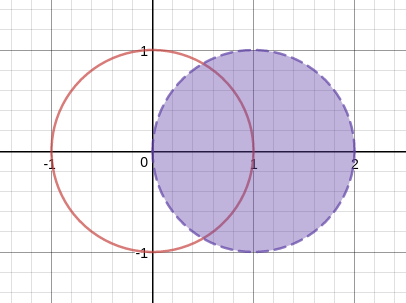
\includegraphics[width=0.25\textwidth]{../images/501_hw5_prob1_fig1}
  \end{center}
  \caption{$S^1$ in red, and $B((1,0),1)$ in purple.}
\end{figure}

By definition, $U$ is open under the subset topology in $\R^2$. Now, consider the preimage $\preimage{f}{U}$. %It is a common result from Geometry that the boundaries of $S^1$ and $B((1,0),1)$ intersect at $(\frac{1}{2},\frac{\sqrt{2}}{2})$ and $(\frac{1}{2},-\frac{\sqrt{2}}{2})$
Since $f$ is a parameterization of the unit circle which begins at $(0,1)$ and proceeds counter-clockwise, approaching $(0,1)$ again as $t\to 1$; then $\preimage{f}{U}=[0,\frac{1}{6})\cup(\frac{5}{6},1)$. We have already shown that intervals of the form $[a,b)$ are not open in the usual topology, thus we have an open set $U$ whose preimage in $f$ is not open. Therefore, $f$ is not continuous, and not a homeomorphism. 
\end{proof}

\pagebreak
\item Prove that the following are both homeomorphic to $\R^2$ with the usual topology: (i.) the open square $\{(x,y) : 0 < x < 1, 0 < y < 1\}$; (ii.) the open ball $B(0,1)$.
\begin{enumerate}[label=(\roman*.)]
\item \begin{proof} Let $S_q$ denote the open square $\{(x,y) : 0 < x < 1, 0 < y < 1\}$. Let $t:[0,1)\to\R$ be defined as $t(x)=\tan(\pi x - \frac{\pi}{2})$. Let $f:S_q\to\R^2$ be defined as $f(x,y)=\left(t(x), t(y)\right)$. 

\begin{figure}[h]
  \begin{center}
    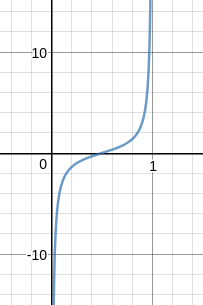
\includegraphics[width=0.25\textwidth]{../images/501_hw5_prob2i_fig1}
  \end{center}
  \caption{$\tan(\pi x - \frac{\pi}{2})$}
\end{figure}

Now, $f$ is a homeomorphism because 
\begin{itemize}
\item $t(x)$ is continuous, since it is a composition of functions which are continuous on $(0,1)$. Also, $\arctan(x)$ is continuous everywhere, so $\inv{t}(x)$ is also continuous by the same reasoning. 
\item $t(x)$ is monotonically increasing, so it is 1-1. 
\item $t(x)$ is onto, since for any real number $x$, one can construct an angle whose tangent is $\pi x + \frac{\pi}{2}$ with two perpendicular segments of length $\pi x + \frac{\pi}{2}$ and 1, respectively. 
\end{itemize}
Thus, $t(x)$ is a continuous bijection whose inverse is also continuous. Therefore, $f$ is a homeomorphism, since it maps each coordinate in $S_q$ to $\R^2$ according to $t(x)$. \end{proof}

\item 
	\begin{proof}
	Let $S_B$ denote the open ball $B(0,1)$. In this proof, it will be convenient to represent points using polar coordinates, so $(r,\theta)$ is the notation we will use. Let $t:[0,1)\to\R$ be defined as $t(x)=\tan(\pi x - \frac{\pi}{2})$, the same as above. Let $f:S_B\to \R^2$ be defined as 
	$$f(r,\theta)=\left(t\left(\tfrac{1}{2}r+\tfrac{1}{2}\right),\theta\right)=\left(\tfrac{\pi}{2}r,\theta\right).$$
	Now, we have already shown that $t$ is continuous, 1-1, and onto, and since $\left(\tfrac{1}{2}r+\tfrac{1}{2}\right)$ is a linear function it also must be a continuous bijection, and clearly so is the identity function. Therefore, since $f$ is a composition of homeomorphisms, then it itself is a homeomorphism. 	
	\end{proof}
\end{enumerate}

\item Let $\Delta = \{(x,x)\}\subset\R^2$. Prove that $\Delta$ as a subspace of $\Rbad^2$ is homeomorphic to $\Rbad^1$. 
\begin{proof}
Let $f:\Delta\to\R^1$ be defined as $f(x,x)=x$. \\
$f$ is clearly 1-1 and onto, since $(a,a)\neq(b,b)\implies a\neq b$, and $\forall x\in \R, \exists (x,x)\in\Delta \mid f(x,x)=x$. Consider any interval $[a,b)$ which is open in $\Rbad^1$. Then, $\preimage{f}{[a,b)}$ is the half-open line segment $\{(x,x): a 
\leq x < b\}=\Delta\cap [a,b)\times[a,b)$. Therefore, $f$ is continuous. 
Now we will show that $F=\inv{f}$ is continuous. $F:\R^1\to\Delta$ is defined as $F(x)=(x,x)$. Let $U$ be any set which is open in $\Delta$. Then, by definition, $U=\Delta\cap [a,b)\times[c,d)$, where $a,b,c,d \in \R$. So, $U=\{(x,x) : \max(a,c) \leq x < \min(b,d)\}$. Now the preimage is $\preimage{F}{U}=\{x : \max(a,c) \leq x < \min(b,d)\}$, which is open in $\Rbad^1$ by definition. Therefore, $F$ is also continuous, and $f$ is a homeomorphism between $\Delta$ as a subspace of $\Rbad^2$ and $\Rbad^1$.
\end{proof}

\pagebreak
\item Let $f : S^2 − \{(0,0,1)\} \to \R^2$ be the function pictured below, that takes a point $(x,y,z)$ to the point $(a,b,0)$ on the $xy$-plane that lies along the line from $(0,0,1)$ to $(x,y,z)$. (This function is called \emph{stereographic
projection}.) Find an explicit formula for $f$, and show that $f$ is a homeomorphism between $S^2 −  \{(0,0,1)\}$ and $\R^2$.

\begin{figure}[h]
  \begin{center}
    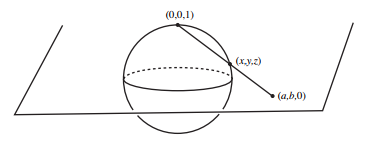
\includegraphics[scale=.80]{../images/501_hw5_prob4_fig1}
  \end{center}
  \caption{Stereographic projection.}
\end{figure}

	\begin{proof}
	By parameterizing the line between $(0,0,1)$ and $(x,y,z)$ and finding the value of $t$ which gives a point on the $xy$-axis, we can obtain the function 
	$$f(x,y,z)=\left(\frac{x}{1-z}, \frac{y}{1-z}, 0\right),$$
	and by parameterizing the line between $(0,0,1)$ and $(a,b,0)$ and finding the value of $t$ which gives a point on the sphere, we can obtain its inverse;
	$$F(a,b,0)=\left(\frac{2a}{a^2+b^2+1}, \frac{2b}{a^2+b^2+1}, \frac{a^2+b^2-1}{a^2+b^2+1}\right).$$
	Now, it can be checked\footnotemark \ that $(F\circ f)(x,y,z)=(x,y,z)$ and $(f\circ F)(a,b,0)=(a,b,0)$, therefore we can conclude that $f$ and $F$ are bijections. Also, since the domain of $f$ is restricted to points in $S^2$, then $(1-z)\neq0$. This means that $f$ is a composition of functions which are continuous on its domain, and thus the function itself is continuous. \\
	Similarly, the domain of $F$ is restricted to the $xy$-plane, and $F$ is a composition of functions which are continuous on its domain (since the denomiator of $F$ is never zero), and thus the function itself is continuous.\\
	Therefore, $f$ is a homeomorphism between $S^2 −  \{(0,0,1)\}$ and $\R^2$.
	\footnotetext{The algebra required for this check is \emph{LONG}, so we have omitted it here. Also, a graphing calculator confirms that this is accurate.}
	\end{proof}
	
\item Which of the following spaces are compact? Explain your reasoning. 
	\begin{enumerate}
	\item $\Rbad^1$\\
	\textbf{Answer:} Not compact, since the collection $\{[-n,n) : n\in\N\}$ is an open cover of $\Rbad^1$ which has no finite subcover. 	
	\item $[-1,1]$ with either-or topology\\
	\textbf{Answer:} Compact, since any open set which contains 0 also contains $(-1,1)$, and now only 2 elements remain. Thus, any open cover of $([-1,1], \textit{either-or})$ has a subcover with at most 3 sets. 
	\item $[0,1]$ as subspace of $\Rbad^1$\\
	\textbf{Answer:} Not compact. First, note that $\{1\}$ is open in this topology, since $[1,2)\cap[0,1]=\{1\}$. Now, $\{[0,1-\frac{1}{n}):n\in\N\}\cup \{\{1\}\}$ is an open cover of the subspace which has no finite subcover.
	\item $\Q\cap[0,1]$, as a subspace of $(\R,usual)$.\\
	\textbf{Answer:} Not compact. Consider $\left\lbrace \Q\cap\left[0,\frac{1}{\Phi}-\frac{1}{n}\right) : n\in\N\right\rbrace\cup\left\lbrace\Q\cap\left(\frac{1}{\Phi}+\frac{1}{n},1\right] : n\in\N\right\rbrace$, where $\Phi$ denotes the irrational number\footnotemark \  $\Phi\approx1.618$ which is the solution to the equation $\inv{\Phi}=\Phi-1$. 
	This collection of sets covers $\Q\cap[0,1]$, but any finite subcollection leaves out rational numbers in the range $\left(\frac{1}{\Phi}-\frac{1}{\max(n)},\frac{1}{\Phi}+\frac{1}{\max(n)}\right)$. 
	\footnotetext{We could have chosen any irrational number between 0 and 1, this one is just my favorite.}
	\end{enumerate}

\setcounter{enumi}{6}
\item Show that an infinite subset of a compact space must have a limit point.
\begin{proof}\textbf{by contradiction}
Let $S$ be an infinite subset of a compact space $X$, and suppose that $S$ has no limit points. Then, for every $x\in S$, $x$ is not a limit point. This means that for each such $x$, there exists an open set $U_x\subset X$ such that $x\in U_x$, and $U_x\cap (S-\{x\})=\emptyset$. Thus, the collection $\{U_x\}_{x\in S}$ is an open cover of $S$ (with respect to the subspace topology) which has no finite subcover, since each $U_x$ is the only set in the collection which contains $x$. This contradicts our assumption that $X$ is compact. 
\end{proof}

\end{enumerate}

\end{document}
